
\section{Velocity models and simulation approach}


The elastic properties ( $P$- and $S$-wave velocities (\vp{} and \vs{}, respectively), and the material's density ($\rho$) of particles) within the domain are require for simulation process and are determined based on the velocity models CVM-S4, CVM-S4.26.2.2.1, CVM-S4.26.2.2.2, and CVM-S4.26.2.2.3 to be evaluated. 

CVM-S4 model integrates available information about the major southern California basins using data from boreholes, oil-well samples, gravity observations, and seismic refraction surveys. The model in itself is built upon empirical rules that use the depths and ages estimated for a set of geological horizons calibrated for southern California. Below and outside the basins, CVM-S4 relies on the 3D seismic tomography model proposed by \citet{Hauksson_2000_JGR}, and an upper-mantle model based on teleseismic inversions introduced into the model by \citet{Kohler_2003_BSSA}.

CVM-S4.26, is a model recently developed by SCEC based on the results from a full 3D tomographic (F3DT) inversion done by \citet{Lee_2014_JGR}. The inversion process involved a sequence of 26 iterations over a reference model extracted from CVM-S4, thus its name. This effort followed the procedure first applied to the Los Angeles region by \citet{Chen_2007_BSSA}. In \citet{Lee_2014_JGR}, the reference model corresponded to a regular grid of 500-m spacing in which the material properties extracted from CVM-S4 were truncated to minimum values of \vpeq{2000}, \vseq{1000} and $\rho$ = 2000 km/m$^3$. The truncation was smoothed until the values extracted from the model reached 3000 m/s, 2000 m/s and 2300 km/m$^3$, respectively. To compute the perturbations to the initial model, \citet{Lee_2014_JGR} used about 38,000 earthquake records and 12,000 ambient noise Green's functions, and combined two inversion methods, the adjoint-wavefield method \citep[AW-F3DT;][]{Tromp_2005_GJI} and the scattering-integral method \citep[SI-F3DT;][]{Zhao_2005_BSSA}. Each iteration in the procedure involved the computation of a forward simulation done using a staggered-grid finite-differences approach \citep{Olsen_1994_Thesis}. The forward simulations were done for a maximum frequency, \fmaxeq{0.2}; and the misfits were computed using seismograms band-pass filtered at 0.02--0.2 Hz. After the 26th iteration perturbations were obtained, the results were merged with the original CVM-S4 model using an interpolation scheme to recover the truncated values. This is the CVM-S4.26 model.

There are currently three alternative CVM-SI.26 models which vary depending on how the perturbations were applied to the original model. These models are:\par
(2.2.1) This model applies an integration scheme in which negative perturbations are only used outside the basins, and positive perturbations are used everywhere.\par
(2.2.2) This scheme applies negative perturbations only if outside the basins, and disregards positive perturbations when inside the basins.\par
(2.2.3) This scheme applies both negative and positive perturbations everywhere, but sets the original value inside the basins as a floor limit.\par

Basin refers to any structure with $V_s < 1000 m/s$ adopting the cutoff value used by Lee et al. (2013) to build the starting model. In all cases, the schemes reverse the process used to build the starting model first, in order to recapture the original structures in CVM-S with values of $V_s < 1000 m/s$, and apply the perturbations later (as described). These schemes have been implemented in the SCEC Unified Community Velocity Model (UCVM) software framework (Gill et al. 2013), which has
already been used to produce unstructured (etree) meshes (Taborda et al., 2007; Tu et al., 2003) at resolutions finer than that used in the inversion. 



\begin{figure*}
    \centering
    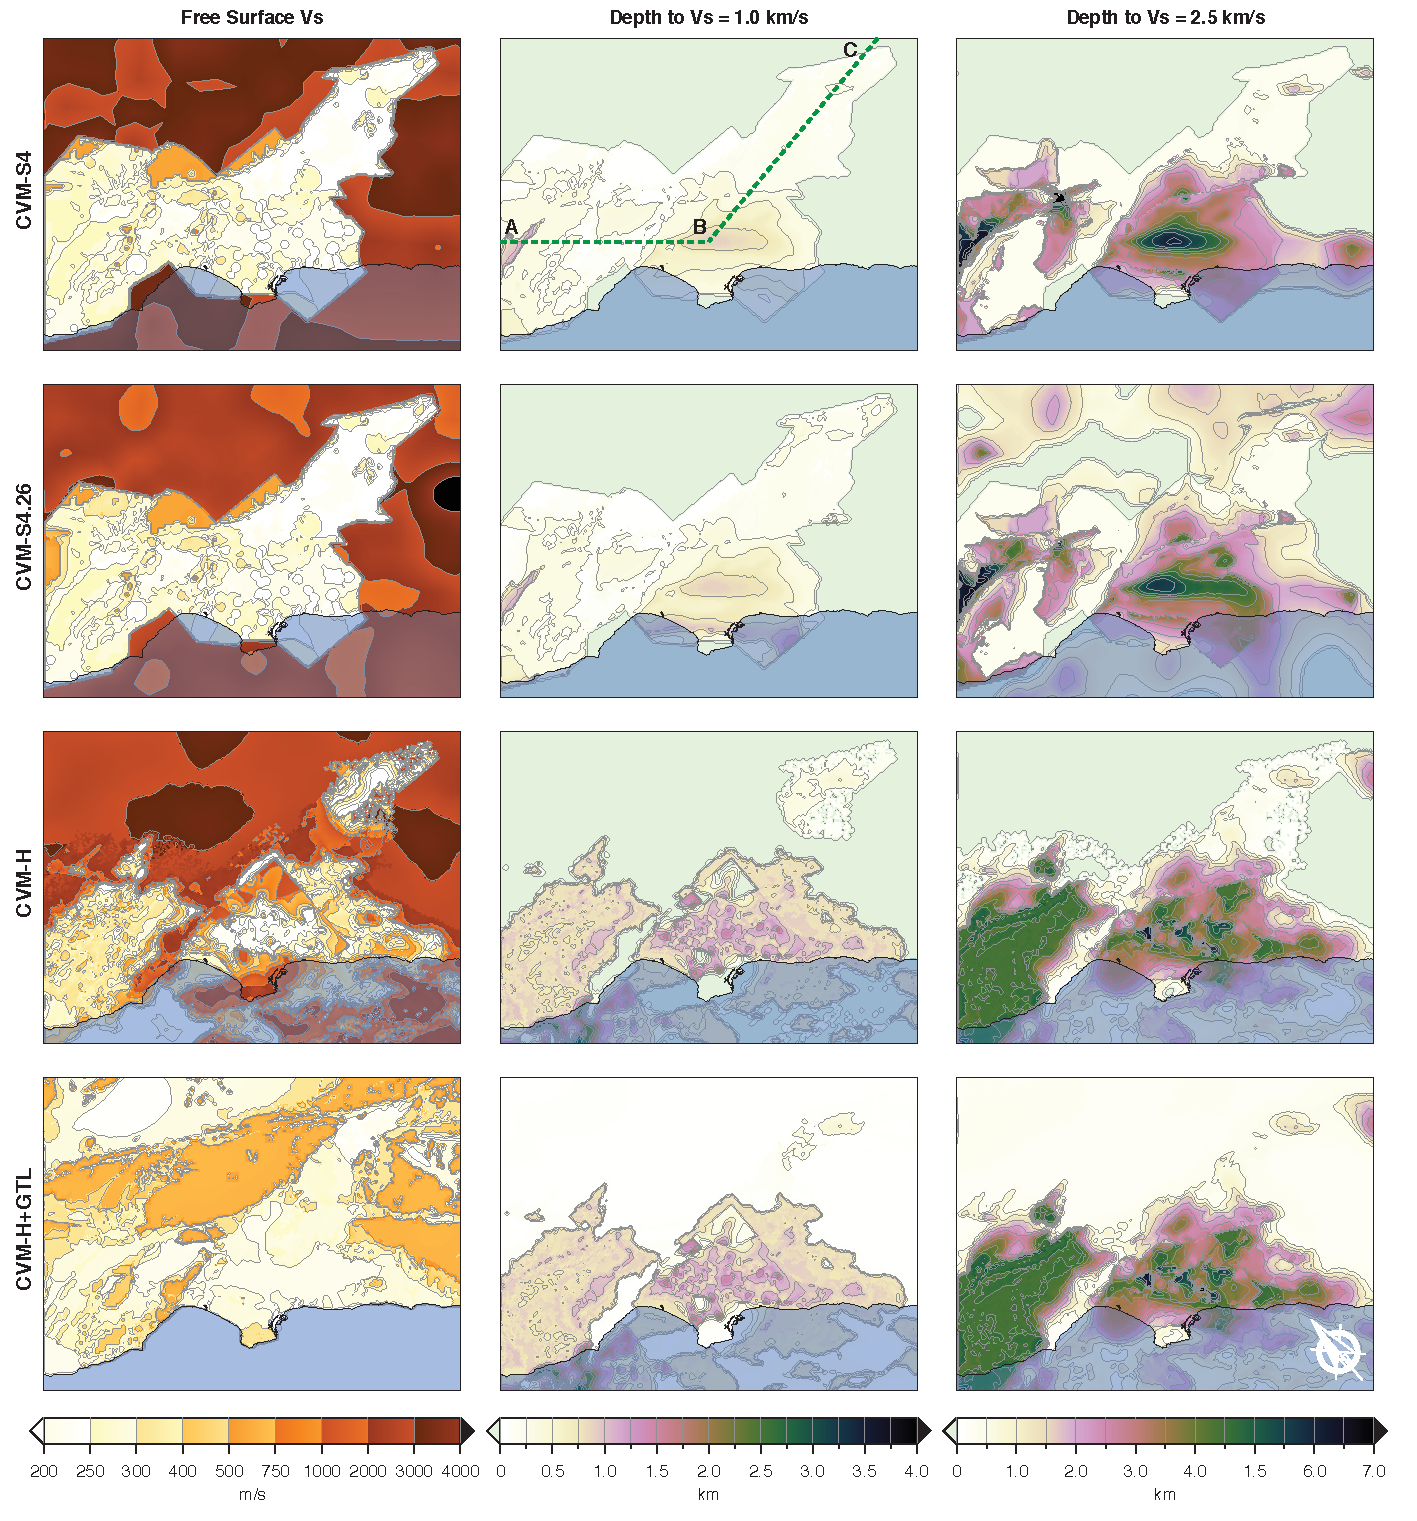
\includegraphics
        [width=\textwidth]
        {figures/pdf/figure-02}
    \caption{Comparison between the southern California community velocity models considered. Left: free-surface shear wave velocity, \vs{}. Center: depth to the isosurface at which \vseq{1000}. Right: depth to the isosurface at which \vseq{2500}. }
    \label{fig:hslices}
\end{figure*}

In all cases, we constructed rasterized versions of the models for the volume simulation domain shown in Fig.~\ref{fig:region}a. This was done using the Unified Community Velocity Model (UCVM) software framework developed by SCEC \citep{Small_2011_AGU, Gill_2015_SSA}, and the UCVM implementation of the etree library \citep{Tu_2003_Tech}, which follows a similar procedure to that described in \citet{Taborda_2007_Proc} and \citet{Schlosser_2008_Proc}.

Fig.~\ref{fig:hslices} shows a comparison between the four models for the free-surface \vs{} and the depths to the isosurfaces at which \vs{} values reach 1.0 and 2.5 km/s. From the isosurfaces, Perhaps the larger contrasts between CVM-S4 and CVM-S4.26 are observed off shore and north of the San Andreas fault, in the Mojave desert (see Fig.~\ref{fig:region} for reference). Other changes are observable in the Santa Clara river valley and Ventura basin, and in the vicinity of the San Bernardino basin, especially to the East (top-right corner of the simulation domain). In all these cases CVM-S4.26 exhibits deeper structures than CVM-S4. Most of the changes in CVM-S4.26 with respect to CVM-S4 are in the deeper structures, and to the north-west of the of segment $\overline{\mathrm{AB}}$ and to the east of segment $\overline{\mathrm{BS}}$.

The simulation is done at maximum frequency of 1 Hz and minumum shear wave velocity of 200 m/s for each earthquake and velocity model combination using Hercules, a parallel 3D finite element computer application for solving forward anelastic wave propagation problems which has been thoroughly tested and verified in multiple supercomputers. Hercules implements an octree datastructure for representing unstructured hexahedral meshes in memory \citep{Tu_2006_Proc} with a solution approach relies on a standard Galerkin method for discretizing the equations of elastodynamics in space, and advances explicitly in time to obtain the next-step state of nodal displacements. The time integration scheme uses first-order backward and second-order central differences to approximate the velocity and acceleration, respectively (Taborda et al. 2010). All simulations are done on Blue Waters at the National Center for Supercomputing Applications.
It is important to note that none of the velocity models provides information about the quality factors \qp{} and \qs{}, which are necessary for modeling the effects of intrinsic attenuation. In this regard, for the case of \qs{}, we adopt the empirical rule
%
\begin{align}
	Q_S =\; 
		& 10.5 - 16 V_S + 153 V_S^2 - 103 V_S^3 
		\nonumber \\
		& + 34.7 V_S^4 - 5.29 V_S^5 + 0.31 V_S^6
	\label{eq:qs}
\end{align}
%
\noindent
used in \citet{Taborda_2013_BSSA, Taborda_2014_BSSA}. This rule is an extension of that proposed by \citet{Brocher_2005_Tech, Brocher_2008_BSSA}, which was in turn inspired by other similar but simpler approximations used in the past \citep[e.g.][]{Olsen_2003_BSSA, Graves_2008_BSSA}. On the other hand, for the case of \qp{}, we use
%
\begin{equation}
	Q_P = \frac{3}{4}\left( V_P / V_S \right)^2 Q_S
	\hspace{.25em},
	\label{eq:qp}
\end{equation} 
% 
which is derived from the special case in which one considers no attenuation due to dilatational deformation, i.e.~$Q_\kappa \rightarrow \infty$ \citep[e.g.,][]{Stein_2003_Book, Shearer_2009_Book}. In both cases we consider the values of $Q$ to remain constant within the range of frequencies considered.

In Hercules, the finite element meshes are built at run-time, and the variable size of the elements is set such that it satisfies the rule
%
\begin{equation}
	e \leq \frac{V_S}{f_{\max} p}
	\hspace{.25em},
	\label{eq:esize}
\end{equation} 
% 
where $p$ is the number of points per wavelength. We set $p=8$ as a minimum requirement, but due to the octree structure of the mesh, for most elements with properties transitioning from one element size to the next, the effective number of points per wavelength varies between 8 and 15.
